%!TEX root = project.tex

\chapter*{About this project}
\paragraph{Abstract}
This is a basic Action Role Playing Game that allows users to manipulate characters and complete a set of actions including moves and attacks. It has life value calculation system to to reflect real-time life value and also allows character to interact with game objects.\\
This application is designed by Unity 3D, the main program languages is C\# and Java. It allows player manipulates character with keyboard to control its move and achieve a set of actions. The Character can be moved by using keyboard "w-a-s-d" to control direction and arrow key "up-down-left-right" can adjust the direction of view.The key "J" is Attack order and key "F" can interact with game objects like communication.\\
This game not only has the player character, it also has monster enemy characters. Monster characters usually patrol on the specific route, once monsters sense there is player character in their detect range, they will catch player and if player out of their range, monsters will back to patrol model. This function is an advanced features, it achieves basic monsters' AI controller.\\
The player character has UI panel to display the information of character and current situation especially the rest of life value, name and level of character.\\
\paragraph{Authors}
Qi Fu



\chapter{Introduction}
PC games, also known as computer games or personal computer games, are video games played on a personal computer rather than a dedicated video game console or arcade machine. Their defining characteristics include a more diverse and user determined gaming hardware and software, and a generally greater capacity in input, processing, and video output.

Home computer games became popular following the video game crash of 1983 leading to the era of the "bedroom coder". In the 1990s, PC games lost mass-market traction to console games before enjoying a resurgence in the mid-2000s through digital distribution.

Newzoo, reports that the PC gaming sector is the third largest (and estimated in decline), with the consoles second largest, and across all platforms as of 2016, 2.2 billion gamers generate US\$101.1 billion in revenue (i.e. all numbers exclude hardware costs), and "Digital game revenues will account for \$94.4 billion or 87\% of the global market. Mobile is the most lucrative segment, with smartphone and tablet gaming growing 19\% year on year to \$46.1 billion, claiming 42\% of the market. In 2020, mobile gaming will represent just more than half of the total games market. China expected to generate \$27.5 billion, or one-quarter of all revenues in 2017." PC is considered synonymous (by them and others) with IBM PC compatible systems; while mobile computers – smartphones and tablets, such as those running Android or iOS – are also personal computers in the general sense. The "APAC" region is estimated to generate \$46.6 billion in 2016, or 47\% of total global game revenues (note, not only "PC" games). China alone accounts for half of APAC's revenues, reaching \$24.4 billion, cementing its place as the largest games market in the world, ahead of the US's anticipated market size of \$23.5 billion. China is expected to have 53\% of revenues from mobile in 2017 (46\% in 2016). The uncoordinated nature of the PC game market and its lack of physical media make precisely assessing its size difficult.\cite{einstein}\\
Types of Game\\
RPG: Role-playing Game is a game in which players assume the roles of characters in a fictional setting. Players take responsibility for acting out these roles within a narrative, either through literal acting or through a process of structured decision-making or character development. Actions taken within many games succeed or fail according to a formal system of rules and guidelines.

WEG: Web Game(Browser Game) is a computer game that is played over the Internet using a web browser. Browser games can be run using standard web technologies or browser plug-ins. The creation of such games usually involves use of standard web technologies as a frontend and other technologies to provide a backend. Browser games include all video game genres and can be single-player or multiple-player. Browser games are also portable and can be played on multiple different devices, web browsers, and operating systems.

ACT: Action Game is a video game genre that emphasizes physical challenges, including hand–eye coordination and reaction-time. The genre includes diverse subgenres such as fighting games, shooter games and platform games which are widely considered the most important action games, though multiple-player online battle arena and some real-time strategy games are also considered to be action games. In an action game, the player typically controls the protagonist or avatar. The avatar must navigate a level, collecting objects, avoiding obstacles, and battling enemies with various attacks. At the end of a level or group of levels, the player must often defeat a boss enemy that is more challenging and often larger than other enemies. Enemy attacks and obstacles deplete the avatar's health and lives, and the player receives a Game over when they run out of lives. Alternatively, the player wins the game by finishing a sequence of levels. But some action games, usually arcade games, are unbeatable and have an indefinite number of levels; and the player's only goal is to maximize their score by collecting objects and defeating enemies.

\chapter{Context}
\begin{itemize}
\item Provide a context for your project.
\item Set out the objectives of the project
\item Briefly list each chapter / section and provide a 1-2 line description of what each section contains.
\item GitHub Link: \href{https://github.com/QiFuChina/RPG}{github.com/QiFuChina/RPG}
\end{itemize}

\section{Filler}
Design Platform
:
Windows Computer
\\
Design Technology
:
Unity 3D, version5.6.4
\\
Design Model
:
Single client service
\\
Game Type
:
A basic Role-Playing Game
\\
Game Model
:
Character, enemy and other objects
\\
Design Inspiration
:
It from a Chinese Wuxia online game.
\\
Function
\\
Manipulate
:
Charater can be moved by using keyboard "w-a-s-d" to control direction, "up-down-left-right" can adjust the direction of view.The key "J" is Attack order and key "F" can interact with game objects like communication.
\\
Modle
:
Character model relative with animation, player press keyboard then model will reflect a set of animation as feedback
\\
Objects
:
Enemy: The enemy has "enemy" target that different with character, when closed to character it will attack Trap: These traps have "enemy" target and cause side-effect to character when triggled them Scene: To allow scenes switch when character go to other environment

\subsection{More filler}


\section{Filler}

\chapter{Methodology}
About one to two pages.
Describe the way you went about your project:
\begin{itemize}
\item Agile / incremental and iterative approach to development. Planning, meetings.
This project aimed at basic functions at first, and then develop the advanced functions with basic functions finished.
\item What about validation and testing? Junit or some other framework.
It can be worked successfully in the windows 10 64bit system. 
\item If team based, did you use GitHub during the development process.
No, this is a individual project, but I am looking forward to use GitHub during team development process.
\item Selection criteria for algorithms, languages, platforms and technolo-gies.
C\# is the widely language that be used in Unity 3D game development industry so that is the reason why I used C\# and Unity 3D to develop this project.
\end{itemize}
\includegraphics[scale=0.5]{img/MainGraph.png} \ref{tikz:graphs}, and the nice diagram in Figure \ref{tikz:mydiagram}.

\begin{figure}
  \centering
  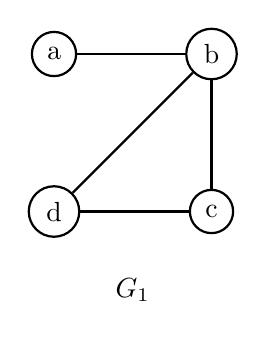
\begin{tikzpicture}
  \begin{scope}[every node/.style={circle,thick,draw}]
  \node (a) at (0,2) {a};
  \node (b) at (2,2) {b};
  \node (c) at (2,0) {c};
  \node (d) at (0,0) {d};
  \end{scope}
  \begin{scope}[every edge/.style={draw=black,thick}]
  \path (a) edge (b);
  \path (b) edge (c);
  \path (b) edge (d);
  \path (c) edge (d);
  \end{scope}
  \node () at (1,-1) {$G_1$};
  \end{tikzpicture}
  \hspace{1.5cm}
  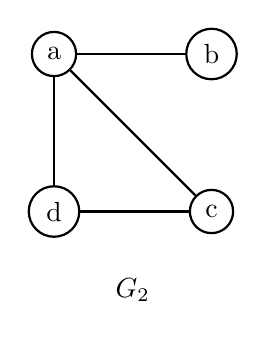
\begin{tikzpicture}
  \begin{scope}[every node/.style={circle,thick,draw}]
  \node (1) at (0,2) {a};
  \node (2) at (2,2) {b};
  \node (3) at (2,0) {c};
  \node (4) at (0,0) {d};
  \end{scope}
  \begin{scope}[every edge/.style={draw=black,thick}]
  \path (1) edge (2);
  \path (1) edge (3);
  \path (1) edge (4);
  \path (3) edge (4);
  \end{scope}
  \node () at (1,-1) {$G_2$};
  \end{tikzpicture}
  \caption{Nice pictures}
  \label{tikz:graphs}
\end{figure}


\begin{figure}
  \centering
  \begin{tikzpicture}[node distance=6cm]
  \node (a) [rect] {A Big Blue Block};
  \node (b) [oval, right of=a] {And His Oval Friend};
  \draw [line] (a) -- (b);
  \end{tikzpicture}
  \caption{Nice pictures}
  \label{tikz:graphs}
\end{figure}


\chapter{Technology Review}
About seven to ten pages.
\begin{itemize}
\item Describe each of the technologies you used at a conceptual level. Standards, Database Model (e.g. MongoDB, CouchDB), XMl, WSDL, JSON, JAXP.
\item Use references (IEEE format, e.g. [1]), Books, Papers, URLs (timestamp) – sources should be authoritative. 
\end{itemize}

\section{XML}
Here's some nicely formatted XML:
\begin{minted}{xml}
<this>
  <looks lookswhat="good">
    Good
  </looks>
</this>
\end{minted}

\chapter{System Design}
As many pages as needed.
\begin{itemize}
\item Architecture, UML etc. An overview of the different components of the system. Diagrams etc… Screen shots etc.
\end{itemize}

\begin{table}[h]
  \centering
  \begin{tabular}{x{2cm}p{3cm}}
    \toprule \\
    Column 1 & Column 2 \\
    \midrule \\
    Rows 2.1 & Row 2.2 \\
    \bottomrule
  \end{tabular}
  \caption{A table.}
  \label{table:mytable}
\end{table}

\chapter{System Evaluation}
As many pages as needed.
\begin{itemize}
\item Prove that your software is robust. How? Testing etc. 
\item Use performance benchmarks (space and time) if algorithmic.
\item Measure the outcomes / outputs of your system / software against the objectives from the Introduction.
\item Highlight any limitations or opportuni-ties in your approach or technologies used.
\end{itemize}

\chapter{Conclusion}
About three pages.

\begin{itemize}
\item Briefly summarise your context and ob-jectives (a few lines).
\item Highlight your findings from the evalua-tion section / chapter and any opportuni-ties identified.
\end{itemize}

